\documentclass[12pt]{article}

% Language setting
\usepackage[english]{babel}

% Set page size and margins
% Replace `letterpaper' with `a4paper' for UK/EU standard size
\usepackage[a4paper,top=2cm,bottom=2cm,left=3cm,right=3cm,marginparwidth=1.75cm]{geometry}

% Useful packages
\usepackage{amsmath}
\usepackage{mathtools}
\usepackage{graphicx}
\usepackage[colorlinks=true, allcolors=blue]{hyperref}
\usepackage{multirow}
\usepackage{xcolor}
\usepackage{colortbl}
\usepackage{algorithm}
\usepackage{algpseudocode}
\usepackage{listings}
\usepackage{tabulary}
\usepackage{multirow}
\usepackage{arydshln}
\usepackage{array}
\usepackage{booktabs}


\usepackage[table]{xcolor}

% definice makra pro české uvozovky
\def\bq{\mbox{\kern.1ex\protect\raisebox{-1.3ex}[0pt][0pt]{''}\kern-.1ex}}
\def\eq{\mbox{\kern-.1ex``\kern.1ex}}
\def\ifundefined#1{\expandafter\ifx\csname#1\endcsname\relax }%
\ifundefined{uv}%
        \gdef\uv#1{\bq #1\eq}
\fi

% Rename caption type name
\makeatletter
\renewcommand*{\ALG@name}{Algoritmus}
\makeatother
\renewcommand{\lstlistingname}{Algoritmus}
\renewcommand{\lstlistlistingname}{Algoritmus}
%====================================================
%========== DEFINITION OF AUTHORS ETC...=============
%====================================================
\title{Solving MWSAT using Genetic Algorithm}
\author{
    Lukáš Tomáš Petrželka 
    % CTU FIT, \\ % Affiliation
}
% \author{Lukáš Tomáš Petrželka}
% \affiliation{Faculty of Information Technology, Czech Technical University in Prague}
\date{20.1.2024}


%====================================================
%========== BEGINNING OF DOCUMENT ===================
%====================================================
\begin{document}
\maketitle

%---------------------------------------------------------------
\vspace*{\fill}
% \begin{abstract}
% Zaměření této práce je pozorovat postup nasazení pokročilé heuristiky. Práce se zaměčuje na heuristiku simulovaného ochlazování pro řešení problému maximální vážené splnitelnosti boolovské formule (MWSAT). Heuristika je odladěná a testovaná s úspěšností 79.93\,\%.
% \end{abstract}
% \vspace*{\fill}
\newpage

%---------------------------------------------------------------
\vspace*{\fill}
\tableofcontents
\vspace*{\fill}
\newpage

%===============================================================
\section{Úvod}

%---------------------------------------------------------------
\subsection{Zadání}

Problém MWSAT (\textbf{M}aximum \textbf{W}eighted \textbf{SAT}isfiability problem) je optimalizační verzí problému booleovské splnitelnosti (SAT). V tomto problému je dána booleovská formule, obvykle v konjunktivní normální formě (CNF), spolu s váhou přiřazenou každé klauzuli. Cílem je určit pravdivostní přiřazení proměnných, které maximalizuje celkovou váhu splněných klauzulí.

Cílem této práce je řešit tento problém pomocí genetického algoritmu a ověřit kvalitu zvolené heuristiky experimentálním vyhodnocením.

\subsection{Data}
Data byly staženy ze \href{https://courses.fit.cvut.cz/NI-KOP/download/index.html#mwsatinst}{stránky předmětu}. Konkrétní vybrané sady instancí použité v tomto projektu jsou v tabulce \ref{tab:data}.

\begin{table}[h]
    \centering
    \begin{tabular}{|c|c|c|c|}
        \hline
        \textbf{Název} & \textbf{Počet proměnných} & \textbf{Počet klauzulí} & \textbf{Obsahuje řešení}\\
        \hline
        wuf20-71 & \texttt{20} & \texttt{71} & Ano \\
        wuf36-157 & \texttt{36} & \texttt{157} & Ano \\
        wuf50-218 & \texttt{50} & \texttt{218} & Ano \\
        wuf75-325 & \texttt{75} & \texttt{325} & Ano \\
        wuf100-430 & \texttt{100} & \texttt{430} & Ne \\
        \hline
    \end{tabular}
    \caption{Dataset}
    \label{tab:data}
\end{table}

\subsection{Implementace}

Genetický algoritmus byl naprogramován v jazyku C++ z důvodu požadavku na optimalizaci. Experimenty a jejich vyhodnocení byly dále provedeny s pomocí jazyku Python. Samotné vizualizace a zkoumané metriky se nacházejí v jupyter notebooku. Celý kód je dostupný \href{https://github.com/LukasTomas/MWSAT}{zde}.

\vspace{1em}
\noindent Níže je uveden výstup nápovědy programu pro řešení MWSAT instance pomocí Genetického Algoritmu:

\begin{figure}[H]
    \centering
    \begin{minipage}[b]{1\textwidth}
        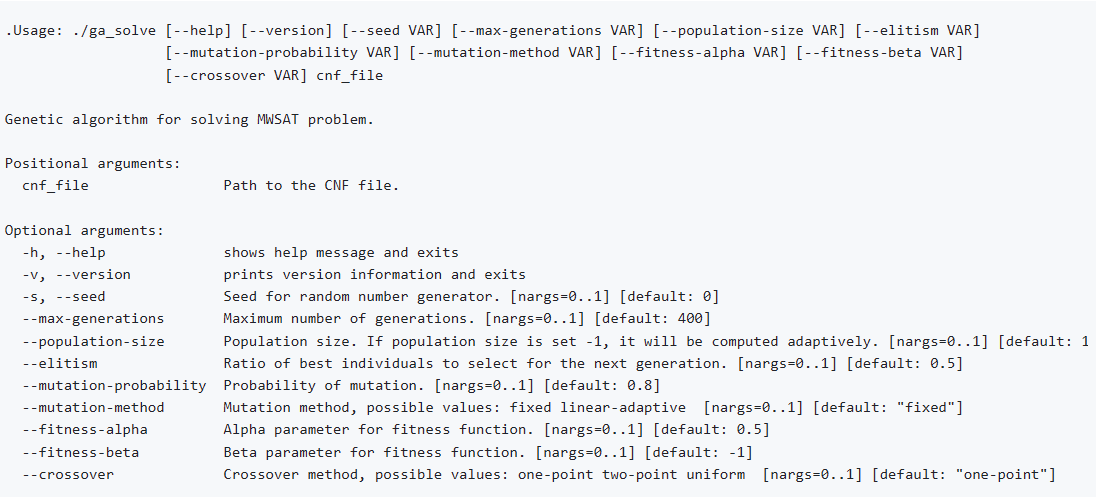
\includegraphics[width=\textwidth]{images/ga_help.png}
        % \caption{Nápověda pro volání programu Genetického Algoritmu pro řešení MWSAT instance.}
        \label{fig:ga_help}
    \end{minipage}
\end{figure}

%---------------------------------------------------------------
\subsection{Základní nastavení genetického algoritmu}
Toto nastavení genetického algoritmu bylo společné pro veškeré iterace white box fáze a i pro black box fázi.

\subsubsection{Genotyp}
Genotypem (reprezentace jedince) je binární řetězec o délce počtu proměnných problému, kde jednotlivé bity představují ohodnocení konkrétních proměnných.

\subsubsection{Inicializace populace}
Populace (množina jedinců) z počáteční generace je inicializována náhodně. Tedy každý jedinec je náhodným binárním řetězcem. Hyperparametr \textit{population size} je laděn ve white-box fázi.

\subsubsection{Selekce}
Krok selekce v genetickém algoritmu určuje, kteří jedinci budou vybráni ke křížení. Byla zvolena \textit{metoda ruletového výběru}. Ta vybere jedince s pravděpodobností proporcionální k jeho fitness hodnotě. Jedinci s vyšší fitness funkcí mají větší šanci na výběr. Jeden jedinec může být vybrán opakovaně.

\subsubsection{Křížení}
Bylo zvoleno \textit{uniformní křížení}, které pro každý bit genotypu výsledného jedince náhodně vybere jednoho z rodičů, od kterého bude tento bit vybrán. 

\subsubsection{Mutace}
Mutace jedinců je provedena tak, že každý bit genotypu je s pravděpodobností \textit{mutation probability} invertován. Hodnota tohoto hyperparametr je také laděna ve white-box fázi.

% \subsubsection{Tvorba další generace}

%===============================================================
\newpage
\section{White box fáze}

Tato fáze slouží k ladění heuristiky s přístupem k algoritmu. Použil jsem v ní převážně datasety s instacemi menší velikosti, a které také mají výsledky: \textit{wuf20-71} a \textit{wuf36-157}. Kromě poslední (5.) fáze, kde jsem použil ještě \textit{wuf50-218}. V každé fázi jsem zvolil kromě sady \textit{M} také \textit{Q}, kde váhy vytvářejí (mírně) zavádějící úlohu. Konkrétně jsem vybral z každé sady 10 instancí.

Pro reprodukovatelnost výsledků jsem zvolil pevně daný seed $123$, který jsem použil k pseudonáhodnému generování několika dalších seedů. Každá instance byla následně spuštěna s jiným seedem. Tímto způsobem do určité míry eliminuji vliv náhodnosti na výsledky algoritmu. Konkrétně jsem v této fázi vygeneroval 5 různých seed hodnot a to z důvodu nedostatku výpočetních prostředků. 

U výsledků sleduji několik metrik. Nejdříve jsem pro každou metriku každou instanci spočítal průměr přes všechny různé seed hodnoty. Následně jsem spočítal průměr přes všechy instance.
\begin{itemize}
    \item \textbf{Poměr splněných klauzulí}
    \item \textbf{Poměr splnění} - počet běhů instance, kde bylo nalezeno řešení, kde ohodnocení dělá formuli           splněnou 
    \item \textbf{Relativní chyba} - $\frac{|S_{\text{optimal}} - S|}{S_{\text{optimal}}}$ - umožňuje srovnávat různé   instance díky normalizaci
    \item \textbf{Hodnota fitness funkce} - pouze u první iterace
\end{itemize}

%---------------------------------------------------------------
\subsection{Iterace 1}

V první iteraci jsem se snažil vymyslet a otestovat fitness funkci.

\begin{table}[h!]
\centering
\caption{Hyperparametry Genetického Algoritmu nastavené v iteraci 1}
\begin{tabular}{@{}ll@{}}
\toprule
\textbf{Parametr}        & \textbf{Hodnota}       \\ \midrule
Max generations           & 1000                \\
Population size           & 300                 \\
Elitism                   & 0.5                 \\
Mutation Probability      & 0.3                 \\
Crossover                 & Uniform             \\
Fitness-alpha             & hledaná                 \\ \bottomrule
\end{tabular}
\label{tab:ga_parameters}
\end{table}

Nejdřive jsem vymyslel tuto první fitness funkci, u které jsem dále zkoumal, jak nastavit hodnotu $\alpha$:
\[
\text{fitness(chromosome)} = \alpha \cdot \frac{C}{\Sigma_C} + (1-\alpha) \cdot \frac{W}{\Sigma_W}
\]
kde jednotlivé proměnné jsou:
\begin{itemize}
    \item $C$ - počet splněných klauzulí
    \item $\Sigma_C$ - počet všech klauzulí
    \item $W$ - suma vah proměnných nastavených na 1
    \item $\Sigma_W$ - suma vah všech proměnných
    \item $\alpha \ in \langle 0, 1 \rangle$ - váhový koeficient určující důležitost maximalizace splněných klauzulí ($C$) oproti maximalizaci váhy proměnných ($W$).
\end{itemize}
Vzhledem k normalizaci výrazů $\frac{C}{\Sigma_C}$ a $\frac{W}{\Sigma_W}$ je možné porovnávat fitness hodnoty řešení na instancích různé velikosti. 

\begin{table}[h!]
\caption{Výsledky testování 1. fitness funkce pro různé hodnoty parametru $\alpha$ u podstady \textit{N}.}
\centering
\renewcommand{\arraystretch}{1.2}
\setlength{\tabcolsep}{10pt}

\def\thickhline{\noalign{\hrule height1.5pt}}
\newcolumntype{?}{!{\vrule width 1.5pt}}

\begin{tabular}{|c?c|c|c|c|c|c|}
\hline
 & \multicolumn{6}{c|}{\textbf{Parametr $\alpha$}} \\ \cline{2-7}
 & 0.15 & 0.30 & 0.45 & 0.60 & 0.75 & 0.90 \\ \thickhline
Poměr splněných klauzulí & 0.939 & 0.959 & 0.977 & 0.993 & 1.000 & 1.000 \\ \hline
Poměr splnění SAT & 0.300 & 0.300 & 0.300 & 0.500 & 1.000 & 1.000 \\ \hline
Relativní chyba & 0.055 & 0.049 & 0.039 & 0.016 & 0.000 & 0.000 \\ \hline
Hodnota Fitness & 0.987 & 0.980 & 0.98 & 0.980 & 0.986 & 0.994 \\ \hline
\end{tabular}

\end{table}

\begin{table}[h!]
\caption{Výsledky testování 1. fitness funkce pro různé hodnoty parametru $\alpha$ u podstady \textit{Q}.}
\centering
\renewcommand{\arraystretch}{1.2}
\setlength{\tabcolsep}{10pt}

\def\thickhline{\noalign{\hrule height1.5pt}}
\newcolumntype{?}{!{\vrule width 1.5pt}}

\begin{tabular}{|c?c|c|c|c|c|c|}
\hline
 & \multicolumn{6}{c|}{\textbf{Parametr $\alpha$}} \\ \cline{2-7}
 & 0.15 & 0.30 & 0.45 & 0.60 & 0.75 & 0.90 \\ \thickhline
Poměr splněných klauzulí & 0.871 & 0.873 & 0.877 & 0.918 & 0.968 & 1.000 \\ \hline
Poměr splnění SAT & 0.000 & 0.000 & 0.000 & 0.000 & 0.100 & 1.000 \\ \hline
Relativní chyba & 0.481 & 0.480 & 0.475 & 0.400 & 0.231 & 0.007 \\ \hline
Hodnota Fitness & 0.981 & 0.961 & 0.942 & 0.930 & 0.935 & 0.969 \\ \hline
\end{tabular}

\end{table}

Následující graf ukazuje, jaký vliv má parametr $\alpha$ na výslednou relativní chybu u obou podsad. Můžeme vidět, že čím větší $\alpha$ tím menší relativní chyba. Jinými slovy, čím více upřednostňuji splnitelnost formule nad maximalizaci vah, tím menší je relativní chyba.
\begin{figure}[H]
    \centering
    \begin{minipage}[b]{0.5\textwidth}
        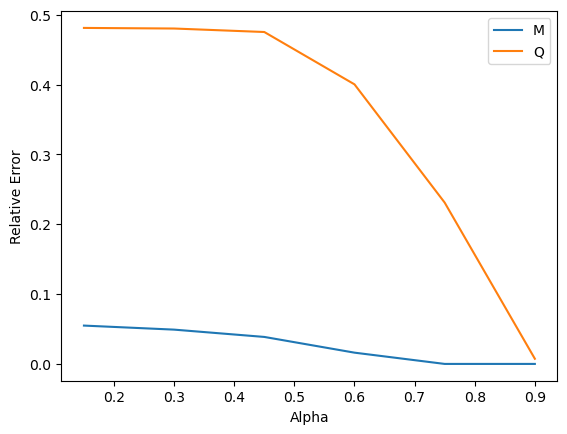
\includegraphics[width=\textwidth]{images/relative_errors_alpha.png}
        % \caption{}
        \label{fig:ga_help}
    \end{minipage}
\end{figure}

%---------------------------------------------------------------


\subsection{Iterace 2}

V této fázi jsem použil stejné parametry jako v předchozí fázi až na jinou fitness funkci, kde jsem se snažil ladit její parametry a zjistit, zda je tato nová fitness funkce lepší než ta v předchozí iteraci.

\begin{table}[H]
\centering
\caption{Hyperparametry Genetického Algoritmu nastavené v iteraci 2}
\begin{tabular}{@{}ll@{}}
\toprule
\textbf{Parametr}        & \textbf{Hodnota}       \\ \midrule
Max generations           & 1000                \\
Population size           & 300                 \\
Elitism                   & 0.5                 \\
Mutation Probability      & 0.3                 \\
Crossover                 & Uniform             \\
Fitness-beta              & hledaná            \\
Fitness-alpha             & hledaná                 \\ \bottomrule
\end{tabular}
\label{tab:ga_parameters}
\end{table}


Upravená fitness funkce je následující:
\[
\text{fitness(chromosome)} = \alpha \cdot \frac{C}{\Sigma_C} + (1-\alpha) \cdot \frac{W}{\Sigma_W} - \beta \cdot \frac{\Sigma_C - C}{\Sigma_C}
\]
Přidaná část je míněna jako penalizace za nesplněné klauzule. Míru penalizace je možné ovlivnit nastavením parametru $\beta$.


\begin{table}[h!]
\caption{Relativní chyba pro různé kombinace parametrů $\alpha, \beta$ u podsady N.}
\centering
\renewcommand{\arraystretch}{1.2}
\setlength{\tabcolsep}{10pt}
\def\thickhline{\noalign{\hrule height1.5pt}}
\newcolumntype{?}{!{\vrule width 1.5pt}}

\begin{tabular}{|c|c?c|c|c|c|}
\hline
 \multicolumn{2}{|c?}{} & \multicolumn{4}{c|}{\textbf{Parametr $\alpha$}} \\ \cline{3-6}
 \multicolumn{2}{|c?}{} & 0.60 & 0.70 & 0.80 & 0.90 \\ \thickhline
\multirow{4}{*}{\textbf{Parametr $\beta$}} & 0.10   & 0.014 & 0.000 & 0.000 & 0.000  \\ \cline{2-6}
 & 0.20                                             & 0.011 & 0.000 & 0.000 & 0.000  \\ \cline{2-6}
 & 0.30                                             & 0.008 & 0.000 & 0.000 & 0.000  \\ \cline{2-6}
 & 0.40                                             & 0.004 & 0.000 & 0.000 & 0.000  \\ \hline
\end{tabular}

\end{table}

\begin{table}[h!]
\caption{Relativní chyba pro různé kombinace parametrů $\alpha, \beta$ u podsady Q.}
\centering
\renewcommand{\arraystretch}{1.2}
\setlength{\tabcolsep}{10pt}
\def\thickhline{\noalign{\hrule height1.5pt}}
\newcolumntype{?}{!{\vrule width 1.5pt}}

\begin{tabular}{|c|c?c|c|c|c|}
\hline
 \multicolumn{2}{|c?}{} & \multicolumn{4}{c|}{\textbf{Parametr $\alpha$}} \\ \cline{3-6}
 \multicolumn{2}{|c?}{} & 0.60 & 0.70 & 0.80 & 0.90 \\ \thickhline
\multirow{4}{*}{\textbf{Parametr $\beta$}} & 0.10   & 0.385 & 0269 & 0.141 & 0.009  \\ \cline{2-6}
 & 0.20                                             & 0.368 & 0.231 & 0.109 & 0.000  \\ \cline{2-6}
 & 0.30                                             & 0.309 & 0.193 & 0.087 & 0.000  \\ \cline{2-6}
 & 0.40                                             & 0.286 & 0.161 & 0.050 & 0.004  \\ \hline
\end{tabular}

\end{table}

Vidíme, že relativní chyba u podsady \textit{Q} pro $\alpha=0.9, \beta=0.3$ je dokonce 0. To je lepší výsledek, než relativní chyba $0.007$ u minulé fitness funkce. Z toho důvodu vybírám tuto fitness funkci i pro další iterace a to právě s parametry $\alpha=0.9, \beta=0.3$.

%---------------------------------------------------------------

\subsection{Iterace 3}

V této iteraci jsem zkoumal, jaký vliv má elitismus (počet nejlepší jedinců ponechaných do další generace bez jakýchkoliv změn) na relativní chybu a poměr splněných klauzulí. Měření jsem provedl na datasetu \textit{wuf20-71} - podsada \textit{M} a \textit{Q}.

\begin{table}[H]
\centering
\caption{Hyperparametry Genetického Algoritmu nastavené v iteraci 3}
\begin{tabular}{@{}ll@{}}
\toprule
\textbf{Parametr}        & \textbf{Hodnota}       \\ \midrule
Max generations           & 1000                \\
Population size           & 300                 \\
Elitism                   & hledaná                 \\
Mutation Probability      & 0.3                 \\
Crossover                 & Uniform             \\
Fitness-beta              & 0.9            \\
Fitness-alpha             & 0.4                 \\ \bottomrule
\end{tabular}
\label{tab:ga_parameters}
\end{table}

\begin{figure}[H]
    \centering
    \begin{minipage}[b]{0.5\textwidth}
        \centering
        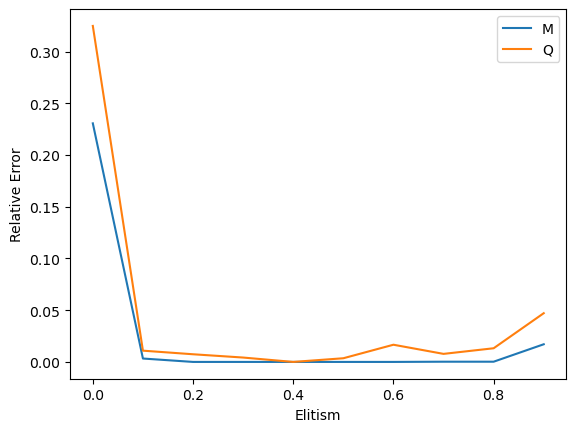
\includegraphics[width=\textwidth]{images/elitism_relative_error.png}
        % \caption{Nápověda pro volání programu Genetického Algoritmu pro řešení MWSAT instance.}
        \label{fig:elitism_relative_error}
    \end{minipage}%
    \hfill
    \begin{minipage}[b]{0.5\textwidth}
        \centering
        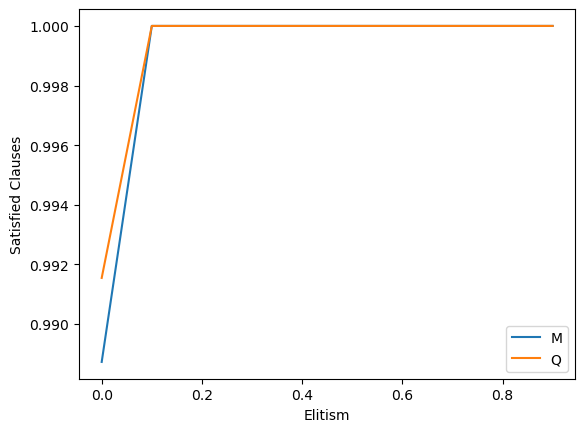
\includegraphics[width=\textwidth]{images/elitism_satisfied_clauses.png}
        % \caption{Nápověda pro volání programu Genetického Algoritmu pro řešení MWSAT instance.}
        \label{fig:elitism_satisfied_clauses}
    \end{minipage}
\end{figure}

Z grafu můžeme vidět, že nejelpších hodnot algoritmus dosáhl při použití elitismu=0.4 (40\% nejlepších jedinců se ponechá do další generace beze změn. Proto jsem pro testování v dalších iteracích zvolil tuto hodnotu tohoto hyperparametru. Testoval jsem to již na těžších instancích, konkrétně na datasetu \textit{wuf36-157}. 
 
%---------------------------------------------------------------

\subsection{Iterace 4}

V této iteraci butu zkoumat optimální nastavení hyperparametru \textit{mutation rate}. Porovnávám fixně nastavenou hodnotu s adaptivní strategií nastavování tohoto hyperparametru.

\begin{table}[H]
\centering
\caption{Hyperparametry Genetického Algoritmu nastavené v iteraci 4}
\begin{tabular}{@{}ll@{}}
\toprule
\textbf{Parametr}        & \textbf{Hodnota}       \\ \midrule
Max generations           & 1000                \\
Population size           & 300                 \\
Elitism                   & 0.4                 \\
Mutation Probability      & variable                 \\
Crossover                 & Uniform             \\
Fitness-beta              & 0.9            \\
Fitness-alpha             & 0.4                 \\ \bottomrule
\end{tabular}
\label{tab:ga_parameters}
\end{table}

Moje navrhnutá lineární adaptivní stratigie pro nastavování pravděpodobnosti mutace:
$$P_{mut}(g) = P_{mut}^{max} - g \cdot \frac{P_{mut}^{max} - P_{mut}^{min}}{G}$$
Kde:
\begin{itemize}
    \item $g$ - číslo aktuální generace
    \item $G$ - číslo maximální generace
    \item $P_{mut}^{max}$ - maximální pravděpodobnost mutace
    \item $P_{mut}^{min}$ - minimální pravděpodobnost mutace (nastaveno na 0.0)
\end{itemize}

Následující graf porovnává fixní strategii a adaptivní. V případě adaptivní strategie hodnota "Mutation Probability" udává startovací pravděpodobnost mutace.

\begin{figure}[H]
    \centering
    \caption{Relativní chyba pro fixní a adaptivní strategii pro pravděpodobnost mutace - podsada \textit{M}.}
    \begin{minipage}[b]{0.5\textwidth}
        \centering
        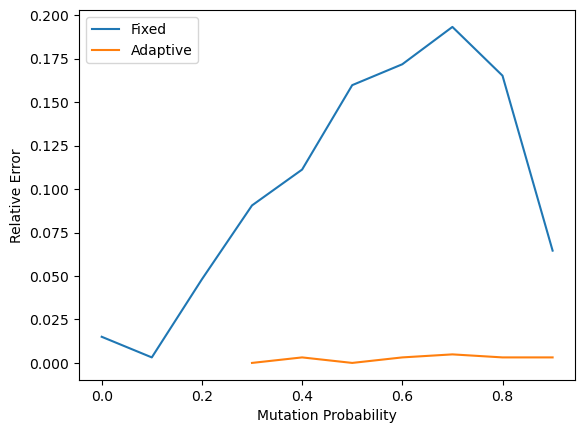
\includegraphics[width=\textwidth]{images/mut_rel_error_M.png}
        % \caption{Nápověda pro volání programu Genetického Algoritmu pro řešení MWSAT instance.}
        \label{fig:elitism_relative_error}
    \end{minipage}%
    \hfill
    \begin{minipage}[b]{0.5\textwidth}
        \centering
        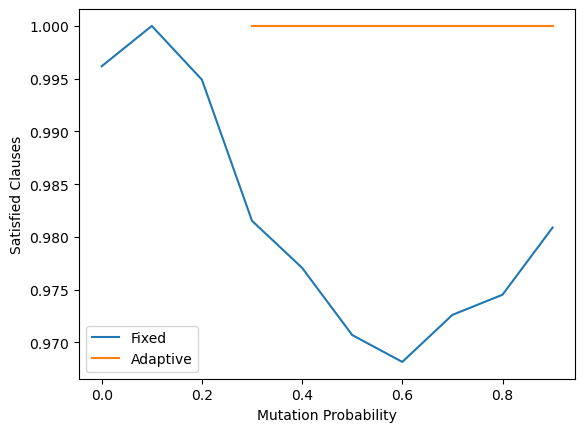
\includegraphics[width=\textwidth]{images/satisfied_rel_error_M.png}
        % \caption{Nápověda pro volání programu Genetického Algoritmu pro řešení MWSAT instance.}
        \label{fig:elitism_satisfied_clauses}
    \end{minipage}
\end{figure}

% \begin{figure}[H]
%     \centering
%     \caption{Relativní chyba pro fixní a adaptivní strategii pro pravděpodobnost mutace - podsada \textit{Q}.}
%     \begin{minipage}[b]{0.5\textwidth}
%         \centering
%         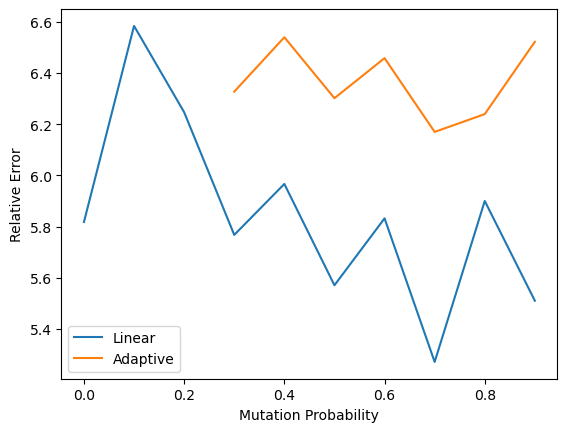
\includegraphics[width=\textwidth]{images/mut_rel_error_Q.png}
%         % \caption{Nápověda pro volání programu Genetického Algoritmu pro řešení MWSAT instance.}
%         \label{fig:elitism_relative_error}
%     \end{minipage}%
%     \hfill
%     \begin{minipage}[b]{0.5\textwidth}
%         \centering
%         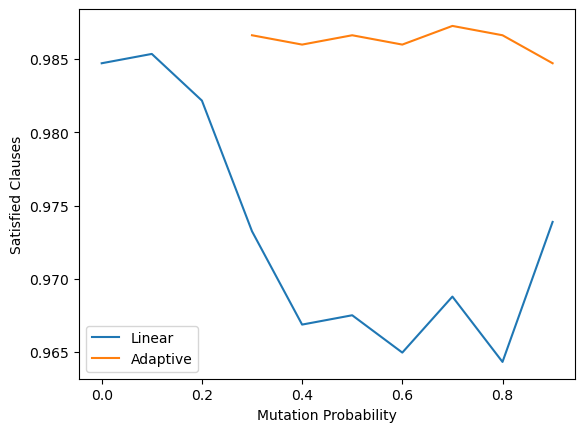
\includegraphics[width=\textwidth]{images/satisfied_rel_error_Q.png}
%         % \caption{Nápověda pro volání programu Genetického Algoritmu pro řešení MWSAT instance.}
%         \label{fig:elitism_satisfied_clauses}
%     \end{minipage}
% \end{figure}

% Narozdíl od předchozích iterací white box fáze je u podsady \textit{Q} relativní chyba násobně větší. To je ale kvůli tomu, že u předchozích iterací jsem používal instance menší velikosti \textit{wuf20-71}, kdežto v této fázi používám \textit{wuf36-157}.

Jelikož adaptivní strategie byla pro různé hodnoty startovací pravděpodobnosti mutace stabilnější, rozhodnul jsem se vybrat tuto strategii.

%---------------------------------------------------------------

\subsection{Iterace 5}

\begin{table}[h!]
\centering
\caption{Hyperparametry Genetického Algoritmu nastavené v iteraci 5}
\begin{tabular}{@{}ll@{}}
\toprule
\textbf{Parametr}        & \textbf{Hodnota}       \\ \midrule
Max generations           & 500                \\
Population size           & laděna             \\
Elitism                   & 0.4 \\
Mutation method           & Linear adaptive \\
Starting Mutation Probability      & 0.7                 \\
Crossover                 & Uniform             \\
Fitness-beta              & 0.9            \\
Fitness-alpha             & 0.4                 \\ \bottomrule
\end{tabular}
\label{tab:ga_parameters}
\end{table}

V poslední páté iteraci jsem se snažil navrhnout funkci \textbf{pro počítání vhodné velikosti populace v závislosti na velikosti problému} (počet proměnných).

Nejprve jsem zjistil průměrné relativní chybu pro sady \textit{wuf20-71}, \textit{wuf36-157} a \textit{wuf50-218} (typ M) v rozmezí hodnot parametru \textit{Population size} od 5 do 200. Jelikož křivky měly velké kratkodobé odchylky, vyhladil jsem je pomocí Savitzky-Golay filtru (používající konvoluci). Vyhlazené křivky jsou vidět na následujícím obrázku \ref{fig:optimal_population_size_smoothed}.

\begin{figure}[H]
    \centering
    \begin{minipage}[b]{0.5\textwidth}
        \centering
        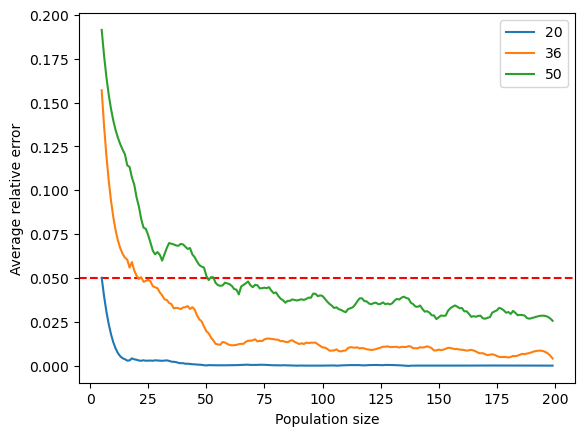
\includegraphics[width=\textwidth]{images/opt_population_size_smooth.png}
        % \caption{Vyhlazené křivky relativních chyb v závislosti na velikosti populace pro různé datové sady instancí.}
        \label{fig:optimal_population_size_smoothed}
    \end{minipage}%
\end{figure}

Dále jsem pro každou datovou sadu zjistil nejmenší hodnotu velikosti populace, aby relativní chyba byla menší než stanovený treshold. Zvolil jsem \textbf{treshold 0.05} jako kompromis mezi přesností a časovými náklady na výpočet.
Dostal jsem následující hodnoty:
\begin{table}[h!]
\centering
\begin{tabular}{|c|c|}
\hline
\textbf{Počet proměnných} & \textbf{Postačující velikost populace} \\ \hline
20                         & 6                          \\
36                         & 21                          \\
50                         & 51                          \\\hline
\end{tabular}
\end{table}

Jelikož v předchozí tabulce nevidím linearitu, rozhodnul jsem se zvolit polynomiální funkci pro počítání vhodné velikosti populace: $P=a \cdot V^b$, kde $a, b$ jsou koeficienty, $V$ je počet proměnných.

Tu jsem nejdřive zlogaritmoval, abych koeficienty mohl odhadnout pomocí lineární regrese (tedy jsem předtím musel zlogaritmovat i hodnoty vstupující do linerání regrese). Dostal jsem hodnoty $a=0.005737$ a $b=2.3115$. Tedy výsledná funkce pro výpočet vhodného počtu jedinců v populaci v závislosti na velikosti problému vypadala takto: $$P = 0.005737 \cdot V^{2.3115}$$ Je však potřeba poznamenat, že jsem pro trénování použil pouze tři datové body. Tento model tedy nemusí být příliš robustní. Nicméně pro účely přibližné aproximace je dostatečný.

Následující tabulka ukazuje spočítaný vhodnou velikost populace pro různý počet proměnných problému:

\begin{table}[h!]
\centering
\begin{tabular}{@{}cc@{}}
\toprule
\textbf{Počet proměnných} & \textbf{Velikost populace} \\ \midrule
20                         & 6                          \\
36                         & 23                          \\
50                         & 49                          \\
75                         & 124                         \\
100                        & 241                         \\ \bottomrule
\end{tabular}
\end{table}



%===============================================================
\newpage
\section{Black box fáze}

\subsection{Úvod}

Tato fáze nasazení slouží k otestování funkčnosti heuristiky se stanovenými parametry. Experiment bude prováděn bez možnosti porozumění vnitřního fungování algoritmu a tím i parametrů heuristiky. 

\subsection{Metody a materiály}
Použil jsem datasety \textit{wuf36-157}, \textit{wuf50-218}, \textit{wuf75-325} a \textit{wuf100-430}, pro každý možnosti \textit{M}, \textit{N} a \textit{Q}. Dataset \textit{wuf100-430} neobsahoval výsledky, takže jsem u něho nemohl počítat relativní chybu. Podobně jako u white box fáze jsem zvolil počet seed hodnot 10 a 100 instancí. Dohromady tedy pro každou datovou sadu proběhlo $10\cdot 100 = 1000$ běhů. Hardware, na kterém byly experimenty provedeny, neumožňoval instanci spustit vícekrát v rozumném časovém úseku. Celkem tedy proběhlo $1000 \cdot 3 \cdot 4 = 12000$ běhů.

Použil jsem takové hodnoty hyperparametrů genetického algoritmu, které jsem zjistil ve white box fázi.
\begin{table}[h!]
\centering
\begin{tabular}{@{}ll@{}}
\toprule
\textbf{Parameter}        & \textbf{Value}       \\ \midrule
Max generations           & 500                \\
Population size           & $P = 0.005737 \cdot V^{2.3115}$             \\
Elitism                   & 0.4 \\
Mutation method           & Linear adaptive \\
Starting Mutation Probability      & 0.7                 \\
Crossover                 & Uniform             \\
Fitness-beta              & 0.9            \\
Fitness-alpha             & 0.4                 \\ \bottomrule
\end{tabular}
\label{tab:ga_parameters}
\end{table}

%---------------------------------------------------------------
\subsection{Výsledky}

\begin{table}[h!]
    \centering
    \caption{Výsledky testovaní v Black box fázi}
    \renewcommand{\arraystretch}{1.2} % Increase row height for better readability
    \begin{tabular}{|l|c|c|c|}
        \hline
        \textbf{Dataset} & \textbf{Splněných klauzule} & \textbf{Splněných formule} & \textbf{Relativní chyba} \\
        \hline
        36-157-M  & $0.9964 \pm 0.0048$ & 0.5700  & $0.0255 \pm 0.0356$ \\
        36-157-N  & $0.9964 \pm 0.0047$ & 0.5600  & $0.0261 \pm 0.0365$ \\
        36-157-Q  & $0.9825 \pm 0.0076$ & 0.0000  & $12.2529 \pm 81.1545$ \\
        50-218-M  & $0.9949 \pm 0.0049$ & 0.3400  & $0.0293 \pm 0.0286$ \\
        50-218-N  & $0.9956 \pm 0.0046$ & 0.3900  & $0.0296 \pm 0.0290$ \\
        50-218-Q  & $0.9811 \pm 0.0077$ & 0.0000  & $8.3406 \pm 37.6638$ \\
        75-325-M  & $0.9875 \pm 0.0050$ & 0.0100  & $0.0514 \pm 0.0358$ \\
        75-325-N  & $0.9886 \pm 0.0050$ & 0.0300  & $0.0529 \pm 0.0368$ \\
        75-325-Q  & $0.9732 \pm 0.0074$ & 0.0000  & $3.6097 \pm 4.8980$ \\
        100-430-M & $0.9821 \pm 0.0047$ & 0.0000  & -- \\
        100-430-N & $0.9823 \pm 0.0048$ & 0.0000  & -- \\
        100-430-Q & $0.9667 \pm 0.0067$ & 0.0000  & -- \\
        \hline
        \textbf{Průměr (M,N)} & $\mathbf{0.9905 \pm 0.0048}$ & $\mathbf{0.2375}$ & $\mathbf{0.0358 \pm 0.0337}$ \\
        \hline
        \textbf{Průměr (vše)} & $\mathbf{0.9856 \pm 0.0057}$ & $\mathbf{0.1583}$ & $\mathbf{2.7131 \pm 2.7117}$ \\
        \hline
    \end{tabular}
    \label{tab:black_box_results}
\end{table}


Z tabulky výsledků \ref{tab:black_box_results} můžeme vidět, že navrhnutá heuristika si umí mnohem lépe poradit s podsadami \textit{M} a \textit{N}, zatímco u podsad \textit{Q}, kde váhy vytvářejí (mírně) zavádějící úlohu, jsou všechny statistiky horší. Průměrná relativní chyba přes všechny datasety navrhnuté heuristiky je 2.7131. Nicméně u podsad \textit{M}, \textit{N} je průměrná relativní chyba 0.0358, což je již výrazně menší.

U všech datasetů je průměrný poměr splněných klauzulí větší než $\sim96\%$. 

%---------------------------------------------------------------

%===============================================================
\newpage\newpage
\section{Závěr}

Implementoval jsem a odladil heuristiku genetického algoritmu pro řešení problému maximální vážené splnitelnosti boolovské formule (MWSAT). 

Nasazená heuristika byla testována na 1200 instancích a celkově proběhlo 12000 běhů. Celková relativní chyba pro lehčí sady (\textit{M}, \textit{N}) je 0.0358 a pro těžší (\textit{Q}) je 2.7131. To hodnotím jako uspokojivý výsledek, ale určitě existují i lepší heuristiky, který by problém řešily s vyšší úspěšností.

\end{document}